%%%%%%%%%%%%%%%%%%%%%%%%%%%%%%%%%%%%%%%%%%%%%%%%%%%%%%%%%%%%%%%%%%%%%%%
% This document is based on the template: Large Colored Title Article %
%                                         Version 1.1 (25/11/12)      %
%                                                                     %
% The template was downloaded from: http://www.LaTeXTemplates.com     %
%                                                                     %
% Original author:                                                    %
% Frits Wenneker (http://www.howtotex.com)                            %
%                                                                     %
% License:                                                            %
% CC BY-NC-SA 3.0 (http://creativecommons.org/licenses/by-nc-sa/3.0/) %
%                                                                     %
% Author of this version:                                             %
% Laura M. Castro (http://www.madsgroup.org/staff/laura)              %
%                                                                     %
% Original licensing terms are maintained                             %
%%%%%%%%%%%%%%%%%%%%%%%%%%%%%%%%%%%%%%%%%%%%%%%%%%%%%%%%%%%%%%%%%%%%%%%

%----------------------------------------------------------------------------------------
%	PACKAGES AND OTHER DOCUMENT CONFIGURATIONS
%----------------------------------------------------------------------------------------

\documentclass[DIV=calc,paper=a4,fontsize=11pt,onecolumn]{scrartcl} % A4 paper and 11pt font size

\usepackage[a4paper,margin=3cm]{geometry} % 2cm margins

\usepackage[galician]{babel} % Galician language/hyphenation
\usepackage[utf8]{inputenc}
\usepackage[protrusion=true,expansion=true]{microtype} % Better typography
\usepackage{amsmath,amsfonts,amsthm} % Math packages
\usepackage[svgnames]{xcolor} % Enabling colors by their 'svgnames'
\usepackage[hang,small,labelfont=bf,up,textfont=it,up]{caption} % Custom captions under/above floats in tables or figures
\usepackage{booktabs} % Horizontal rules in tables
\usepackage{fix-cm}   % Custom font sizes - used for the initial letter in the document

\usepackage{sectsty}  % Enables custom section titles
\allsectionsfont{\usefont{OT1}{phv}{b}{n}} % Change the font of all section commands

\usepackage{fancyhdr} % Needed to define custom headers/footers
\pagestyle{fancy}     % Enables the custom headers/footers
\usepackage{lastpage} % Used to determine the number of pages in the document (for "Page X of Total")

% Headers - all currently empty
\lhead{}
\chead{}
\rhead{}

% Footers
\lfoot{\textsc{vvs-informe-prácticas}}
\cfoot{}
\rfoot{\footnotesize Páxina \thepage\ de \pageref{LastPage}} % "Page 1 of 2"

\renewcommand{\headrulewidth}{0.0pt} % No header rule
\renewcommand{\footrulewidth}{0.4pt} % Thin footer rule

\definecolor{UDC}{RGB}{206,0,124}
\definecolor{DarkUDC}{rgb}{0.75,0.75,0.75}
\definecolor{LightUDC}{RGB}{128,128,128}

\usepackage{lettrine} % Package to accentuate the first letter of the text
\newcommand{\initial}[1]{ % Defines the command and style for the first letter
\lettrine[lines=3,lhang=0.3,nindent=0em]{
\color{UDC}
{\textsf{#1}}}{}}

%----------------------------------------------------------------------------------------
%	TITLE SECTION
%----------------------------------------------------------------------------------------

\usepackage{titling} % Allows custom title configuration

\newcommand{\HorRule}{\color{UDC} \rule{\linewidth}{1pt}} % Defines the pink horizontal rule around the title

\pretitle{\vspace{-30pt} \begin{flushleft} \HorRule \fontsize{20}{20} \usefont{OT1}{phv}{b}{n} \color{DarkUDC} \selectfont} % Horizontal rule before the title

\title{INFORME DE PRÁCTICAS} % Your article title

\posttitle{\par\end{flushleft}\vskip 0.5em} % Whitespace under the title

\preauthor{\begin{flushleft}\large \lineskip 0.5em \usefont{OT1}{phv}{b}{sl} \color{DarkUDC}} % Author font configuration

\author{Repositorio del proyecto: \\
\begin{itemize}
	\item https://github.com/andreu-barro/VVS-DFA-JAVA \\
	\item https://github.com/srjavimoure/VVS-DFA-C \\
\end{itemize}
Participantes del proyecto: \\
\begin{itemize}
	\item F. Javier Moure López, \\
	\item Emma Oitavén Carracedo, \\
	\item Xoan Andreu Barro Torres \\
\end{itemize}
}

\postauthor{\footnotesize \usefont{OT1}{phv}{m}{sl} \color{Black} % Configuration for the institution name
\par\end{flushleft}\HorRule} % Horizontal rule after the title

\date{\sffamily Validación e Verificación de Software} % Add a date here if you would like one to appear underneath the title block

%----------------------------------------------------------------------------------------

\usepackage{graphicx}
\usepackage{hyperref}
\hypersetup{colorlinks=true,
            allcolors=UDC}

\usepackage{array}
\usepackage{colortbl}

%----------------------------------------------------------------------------------------

\newcommand{\hint}[1]{\begin{quote}\itshape #1 \end{quote}}

%----------------------------------------------------------------------------------------

\begin{document}

\maketitle % Print the title
\thispagestyle{fancy} % Enabling the custom headers/footers for the first page 
\clearpage

%----------------------------------------------------------------------------------------
%	ARTICLE CONTENTS
%----------------------------------------------------------------------------------------

\section{Descripción del proyecto}

Aplicación que modifica un Autómata Finito Determinista (DFA), eliminando estados y transiciones superfluas de modo que devuelva un DFA equivalente más sencillo. \\

Esta aplicación fue realizada en los lenguajes de programación Java y C.

\section{Estado actual}

	Nuestra aplicación se divide en los siguientes módulos:
	\begin{itemize}
		\item Clase \textit{State}: Representación de un estado del autómata.
		\item Clase \textit{Symbol}: Representación de un símbolo del lenguaje aceptado por el autómata.
		\item Clase \textit{GenList}: Implementación de una lista de elementos de tipo no predeterminado
		\item Clase \textit{Alphabet}: Lista de símbolos de un lenguaje, Alfabeto del autómata.
		\item Clase \textit{Transition}: Lista de transiciones del autómata. Contienen un estado inicial, un estado final y un símbolo de transición.
		\item Clase \textit{DFA}: La representación del autómata. Implementación de varias funcionalidades como obtención de estados conectados, generación de autómata a partir de una cadena de texto, y más.
	\end{itemize}
	
	El objetivo es probar que todas estas módulos funcionan correctamente, para ello aplicaremos pruebas de unidad, pruebas dinámicas, pruebas de rendimiento y chequearemos el estilo de programación.
	Una vez usemos las diversas herramientasa nuestra disposición, como por ejemplo cobertura y PIT (Java) o lcov y Unity (C), podremos demostrar que nuestra aplicación, y los módulos que la componen, son correctos y estables y dispondremos de una serie de pruebas para demostrarlo. 

\section{Especificación de pruebas}

\textit{Para el repositorio de Java}: Ir a doc/Informe/Informes. \\

\textit{Para el repositorio de C}: Ir a doc/ \\

En cada documento se encuentra la descripción de las pruebas a realizar, describiendo la entrada proporcionada, salida esperada (lo cual consideramos nuestro criterio de éxito), función a probar y el tipo de prueba, todas ellas divididas primero en documentos por cada clase de prueba (unidad, integración,...) y segundo en apartados según el módulo. \\

Para referencia y facilidad de búsqueda, cada prueba cuenta con un código de identificación, referenciado tanto en los documentos de especificación de pruebas como en el código (p.ej. \textit{JAVA-SYM-NEW-01}). \\

Las pruebas definidas son comunes a ambos lenguajes, con añadidos concretos necesarios según la idiosincracia propia de cada lenguaje de programación. \\

\section{Registro de pruebas}
\subsection{Pruebas unidad: JUnit y Unity}
Estas herramientas se utilizan para realizar pruebas unitarias sobre nuestra aplicación, nos sirven para encontrar errores y solventar los problemas en la programación de forma manual.
Se realizan pruebas de todas las funciones implementadas en la aplicación.
Los casos de prueba se implementan manualmente como parte de funciones de prueba, utilizamos la directiva assertEqual(Expected, Expr).

\subsection{Pruebas de unidad: Mockito y CMock}
Para poder crear un buen conjunto de pruebas unitarias, es necesario que nos centremos exclusivamente en la clase a testear, simulando el funcionamiento de las capas inferiores (pensad por ejemplo en olvidarnos de la capa de acceso a datos, DAO). De esta manera estaremos creando test unitarios potentes que nos permitiría detectar y solucionar los errores que tengamos o que se cometan durante el futuro del desarrollo de nuestra aplicación.
Para esta tarea nos apoyaremos en el uso de mock objects, que no son más que objetos que simulan parte del comportamiento de una clase. \\

Los mocks son sólo necesarios para los módulos Transition, Alphabet, y DFA, pues dependen de otros módulos para su funcionamiento.

\subsection{Pruebas basadas en propiedades: Quickcheck y QuickCheck4c}
QuickCheck es una  herramienta para generar automáticamente y ejecutar casos de prueba aleatorios, basados en especificaciones de propiedades. Es decir, ejecutar pruebas con esta herramienta, significa instanciar las propiedades n veces. Las pruebas se detienen al encontrar un caso concreto en el que la propiedad no se cumple (contraejemplo). La ejecución con éxito significa que ninguno de los casos generados incumplió la propiedad. \\
Se crean generadores de:
\begin{itemize}
	\item GeneradorAlphabet
	\item GeneradorDFA
	\item GeneradorState
	\item GeneradorSymbol
	\item GeneradorTransition
	\item GeneradorGenList
\end{itemize}

\textit{Java}: La programación de generadores para aplicar Quickcheck se realiza en el siguiente paquete: es.udc.fic.vvs.vvsproject.generadorTest \\

\textit{C}: Las pruebas de QCC se ejecutan independientemente de las de Unity. Se pueden encontrar en los archivos con nombre modulo-qcc.c

\subsection{Validación de calidad de las pruebas: Cobertura y lcov}
Estas herramientas nos permiten comprobar qué parte del código estamos cubriendo con nuestras pruebas, revelando partes del código pendientes de prueba y permitiéndonos hacer pruebas más exhaustivas. \\
De esta forma Cobertura se convierte en una potente herramienta de trabajo, ya que lo podemos usar como medida de calidad (mientras más código tengamos probado, más garantías tenemos de que cubrimos todos nuestros casos de uso).
Nuestro objetivo es llegar a cobertura cercana al 100\% para nuestros módulos.

\subsection{Pruebas no funcionales: JETM}
JETM permite realizar pruebas de rendimiento y comprobar la velocidad de ejecuciones al implementar unas pruebas con n iteraciones. Se pueden generar test con múltiples iteraciones para detectar problemas de rendimiento. \\

Pruebas que se realizarán en el paquete es.udc.vvs.dfa.rendimiento \\

En C, nos valdremos del comando \textit{time} en consola de comandos para determinar los tiempos de ejecución de la aplicación compilada bajo distintas estrategias de optimización de código.

\subsection{Validación de calidad de las pruebas (mutación testing): PIT y Milu}

El  método que utilizaban en el sistema para realizar estas mediciones lo denominaba “Programa mutado”.
Básicamente, el Mutation testing consiste en introducir pequeñas modificaciones en el código fuente de la aplicación, a las que denominaremos mutaciones o mutantes.

Si las pruebas pasan al ejecutarse sobre el mutante, el mutante sobrevive.
Si las pruebas no pasan al ejecutarse sobre el mutante, el mutante muere
El objetivo es que todos los mutantes mueran, así podremos decir que el test responde a la definición concreta del código y que lo prueba correctamente.
Este concepto se basa en dos hipótesis:
\begin{itemize}
	\item Hipótesis del programador competente: La mayoría de los errores introducidos por programadores Senior consisten en pequeños errores sintácticos.
	\item Hipótesis del efecto de acoplamiento: Pequeños fallos acoplados pueden dar lugar a otros problemas mayores.
\end{itemize}
Problemas de mayor orden serán revelados por mutantes de mayor orden, que se crean mediante la unión de multiples mutaciones.

\subsection{Pruebas estructurales: CheckStyle y CPPCheck}

Checkstyle es una herramienta de desarrollo que ayudar a los programadores a escribir código Java para que se adhiera a un estándar de codificación. Automatiza el proceso de comprobación de código Java. Esto lo hace ideal para los proyectos a los que se desea aplicar un estándar de codificación.

Checkstyle es altamente configurable y se puede hacer para apoyar casi cualquier estándar de codificación. De tal manera que se puedan suministrar diferentes estándares de código para su posterior comprobación mediante la herramienta.

Reglas del CheckStyle
El conjunto de reglas disponible es muy completo y está clasificado en los siguientes grupos:
\begin{itemize}
	\item Comentarios Javadoc: facilitar el mantenimiento pasa por comentar el código, pero luego los comentarios también hay que mantenerlos... CheckStyle tiene muchas reglas para los javadoc y es muy flexible. Te permite, por ejemplo, obligar a comentar los nombres de clases, todos los métodos menos los get/set y los atributos públicos.
	\item Convenciones de nombres: puedes definir una expresión regular para el nombre de todo. 
	\item 	Cabeceras: expresiones regulares para la cabecera de los ficheros.
	\item Imports: reglas para los import, como no usar *, imports sin usar, etc.
	\item Violaciones de tamaño: define un máximo para el tamaño de tus clases, métodos, líneas y número de parámetros de un método.
	Espacios en blanco: un montón de reglas para definir donde se ponen espacios en blanco y tabuladores en el código.
	\item Modificadores: establece un orden para los modificadores y evita modificadores innecesarios.
	\item Bloques: reglas para los bloques de código y sus llaves.
	\item Problemas en la codificación: Acá hay de todo, desde malas prácticas tipo asignaciones internas y posibles fuentes de bugs como definir un método equals que no es el equals(Object), a cosas más estéticas o poco prolijas, como que el default sea el último elemento en un switch o paréntesis innecesarios.
	\item Diseño de clases: varias reglas sobre el diseño de interfaces y clases, con especial atención en las excepciones.
	\item Duplicados: te permite definir un mínimo de líneas para buscar código duplicado en tus clases.
	\item Métricas: define máximos para métricas como complejidad ciclomática, complejidad de expresiones lógicas, npath, líneas de código seguidas sin comentar y dependencia de clases.
	\item Misceláneo: variables final, indentación, un buscador de expresiones regulares y varias cosas más.
	\item J2EE: reglas para EJBs.
	\item Otros: internos a CheckStyle y activados por defecto.
	\item Filtros: para eventos de auditoria del propio CheckStyle, no hace falta mirarlos.
\end{itemize}	


\textit{C}: Por parte de C, CppCheck realiza otras comprobaciones como vigilar la petición y liberación de memoria dinámica, advirtiendo de fugas potenciales de memoria así como cualquier uso peligroso de un puntero.


\section{Registro de errores}
\subsection{Pruebas unidad: JUnit y Unity}
Se puede comprobar que no fallan.

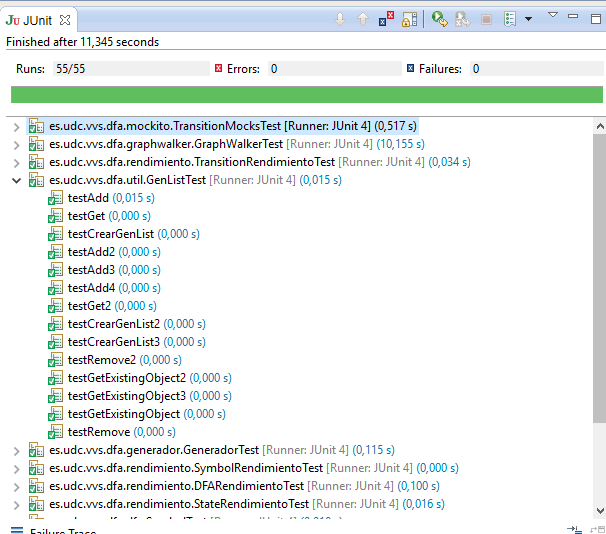
\includegraphics[width=15cm]{Imagenes/junit.png} \\

\textit{C:} La mayoría de issues encontradas se deben a un uso incorrecto de punteros. La mayoría de ellos ni siquiera llegaba a fallar el error, simplemente los tests paraban con un segmentation fault, lo cual llevó a la búsqueda manual del problema.
	
\subsection{Pruebas dinámicas de unidad: Mockito y CMock}
Se puede comprobar que no fallan.

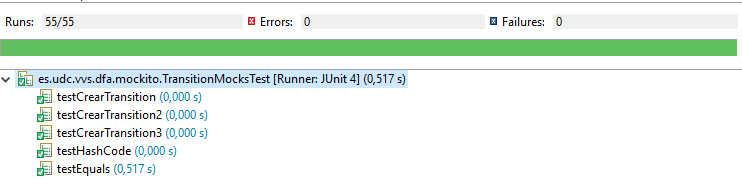
\includegraphics[width=15cm]{Imagenes/mockito.png} \\
	
\textit{C:} No fue posible emplear esta herramienta.
	
\subsection{Validación de la calidad de las pruebas: Cobertura y lcov}

Estado inicial:


	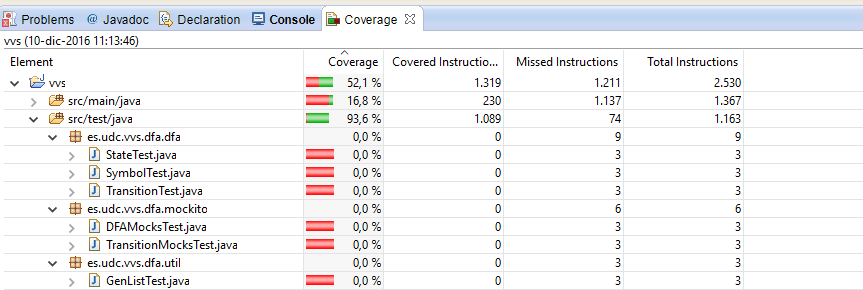
\includegraphics[width=15cm]{Imagenes/sinCobertura.png}


Estado final:

Hemos realizado aumentado las pruebas en GenList para mejorar la cobertura de las pruebas, por definición habíamos decidido no realizar pruebas sobre DFA porque considerábamos que el funcionamiento de DFA estaba incluido en GenList.

	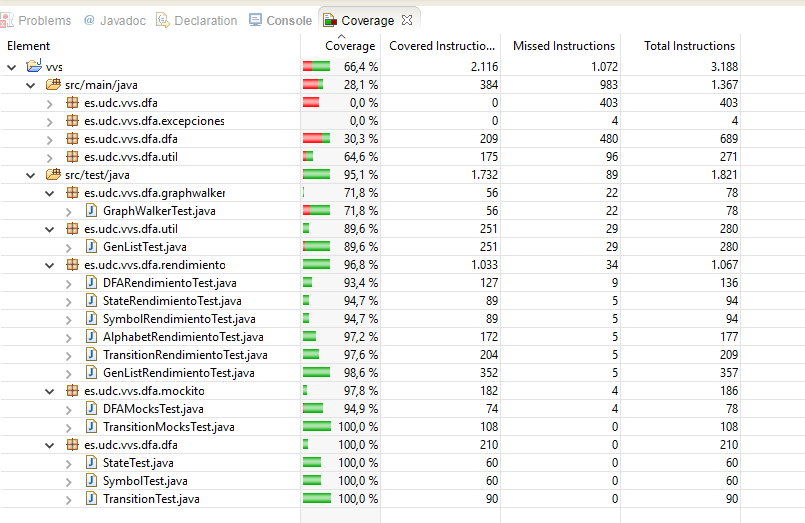
\includegraphics[width=15cm]{Imagenes/Cobertura.png}

\textit{C:} Se puede generar el informe con "make doc". En la carpeta doc, se encontrará una carpeta llamada coverage la cual contiene el informe de cobertura de las pruebas:

	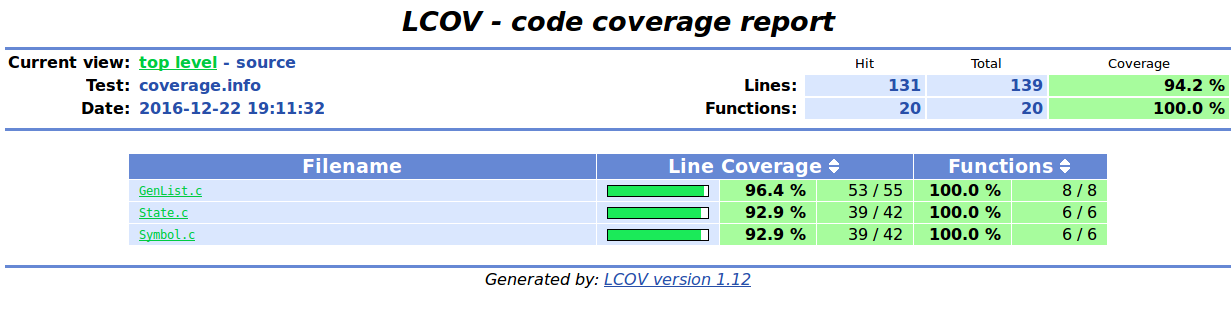
\includegraphics[width=16cm]{Imagenes/lcov2.png} \\

\subsection{Pruebas no funcionales: JETM}
Resultado del rendimiento de JETM:
%\href{Informes/SiteTestInicial/jetm-timing-report.html}{Informe JETM} \\

	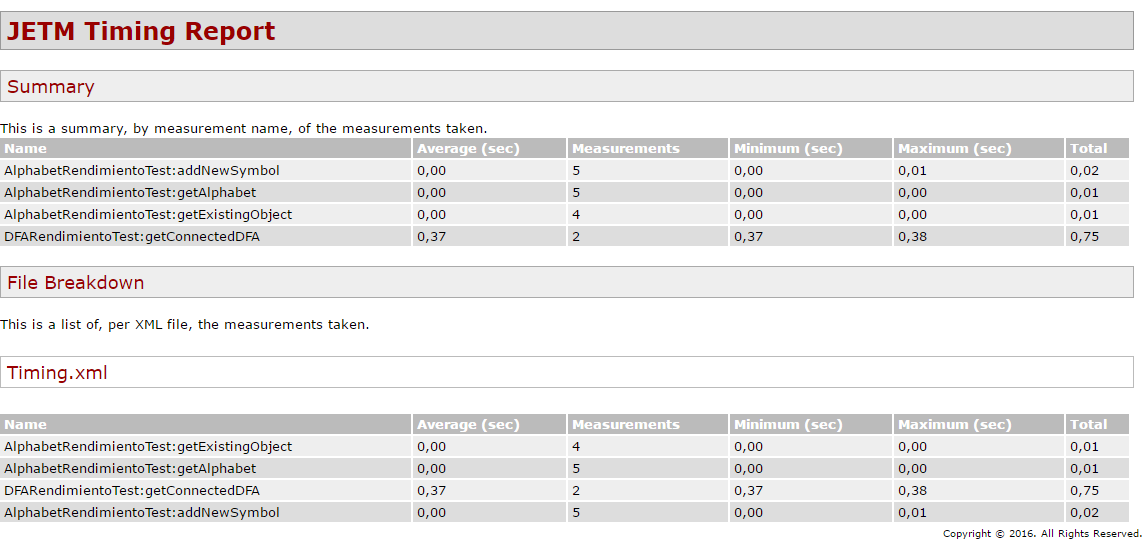
\includegraphics[width=16cm]{Imagenes/JEMReport.png} \\
%	\includegraphics[width=16cm]{Imagenes/JETM2.png} \\
Con JETM hemos tenido problemas  a la hora de que nos genera el site todos los resultados de las pruebas. Sí genera los resultados guardandolos en un xml con todos los resultados, pero no los muestra en la página de resultados del site.
%	Consideramos que el rendimiento es bueno.
\subsection{Validación de calidad de las pruebas (mutation testing): PIT y Milu}
Realizado el mutation testing, resultados:

\href{Informes/pit-reports/index.html}{Informe PIT} \\

\textit{C:} No se logró usar Milu para hacer mutation testing.

\subsection{Pruebas estructurales: CheckStyle}
	Al pasar la herramienta de CheckStyle descubrimos que nuestra aplicación tiene muchos errores de estilo, es decir, que no cumple el estándar de programación java.
	
	Resumen de errores encontrados:
	\begin{itemize}
		\item Faltan comentarios: En la mayoría de clases faltan comentarios javadoc. Se añaden.
		\item Mala indexación código y espacios: Se reestructura el código para que solventar dichos errores.
	\end{itemize}
	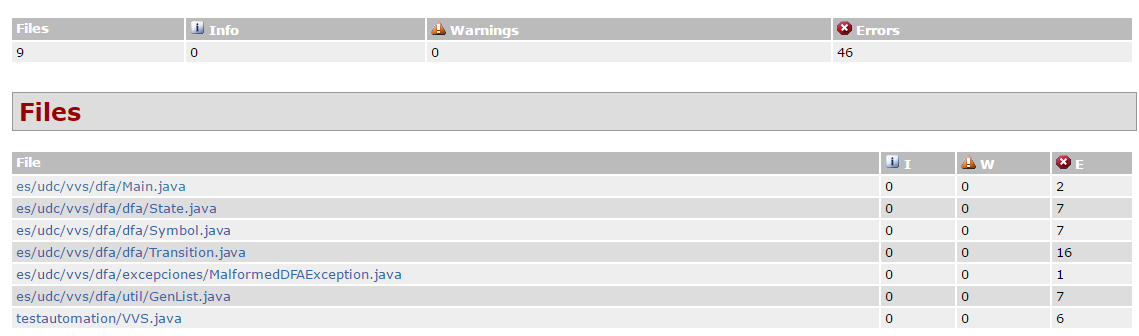
\includegraphics[width=15cm]{Imagenes/erroresCheckStyle.png} \\
	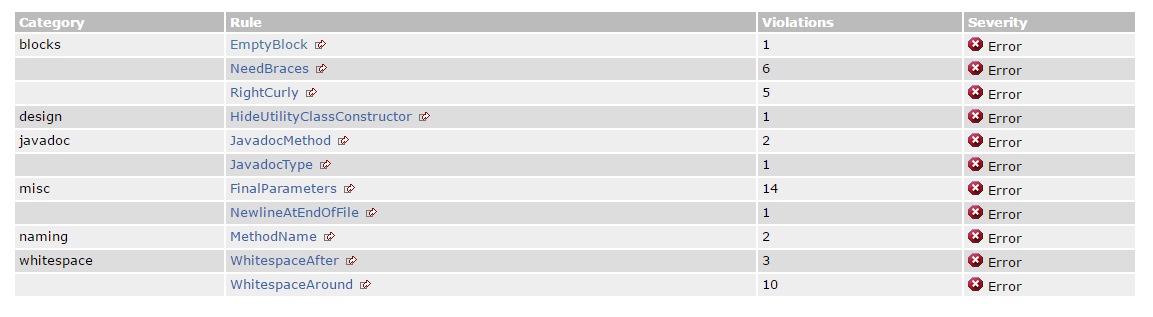
\includegraphics[width=15cm]{Imagenes/checkStyleErrores.png} \\
	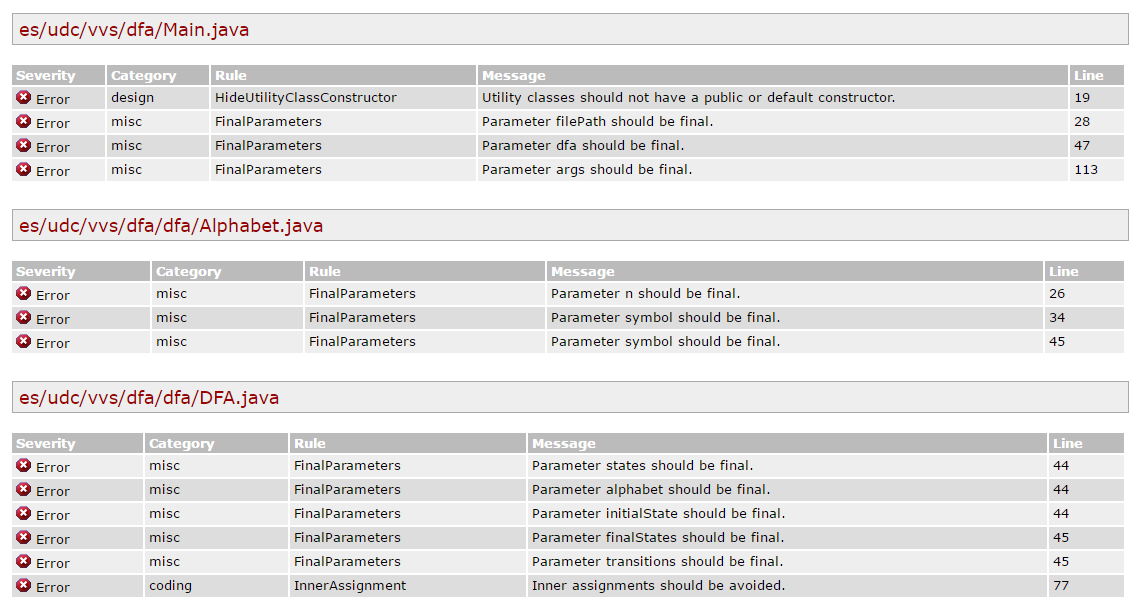
\includegraphics[width=15cm]{Imagenes/checkStyleErrores1.png} \\
	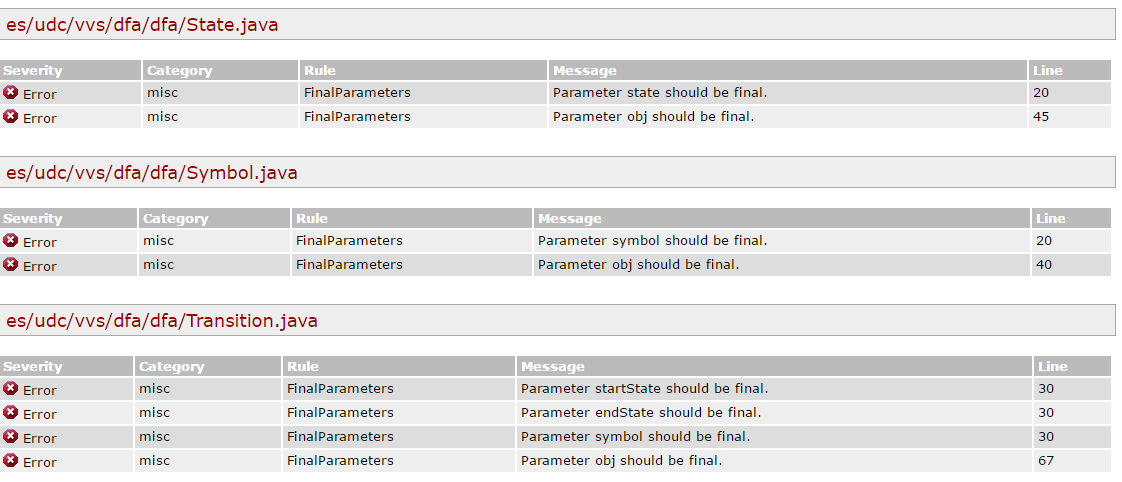
\includegraphics[width=15cm]{Imagenes/statecheckstyle.png} \\
	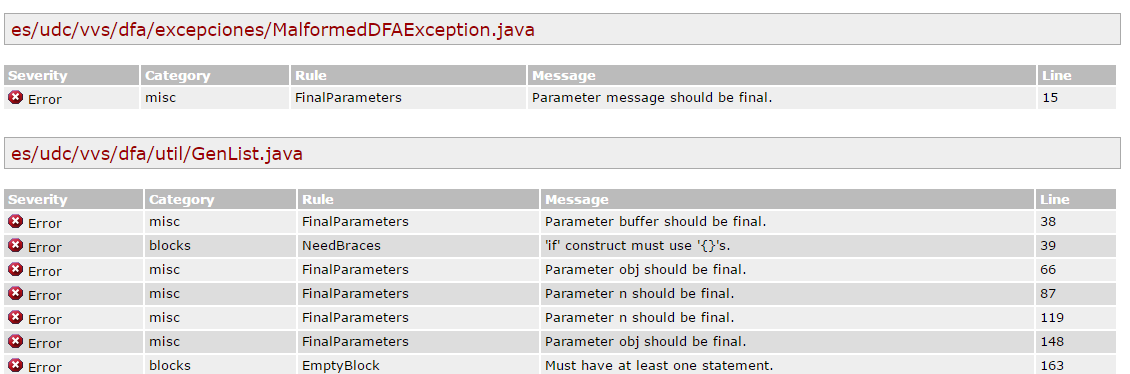
\includegraphics[width=15cm]{Imagenes/checkStyleErrores3.png} \\
	Después de revisar los errores encontrados, resolvemos los errores de estilo encontrados y este es el resultado:
	  \href{Informes/checkStyle-report/checkstyle.html}{Informe CheckStyle} \\
	
	\subsection{Pruebas estáticas/estructurales: FindBugs y CppCheck}
	
	FindBugs es un programa que utiliza el análisis estático para buscar errores en el código de Java.
	
	\href{Informes/findBugs-report/findbugs.html}{Informe Find bugs} \\
	
	Errores encontrados inicialmente:
	
	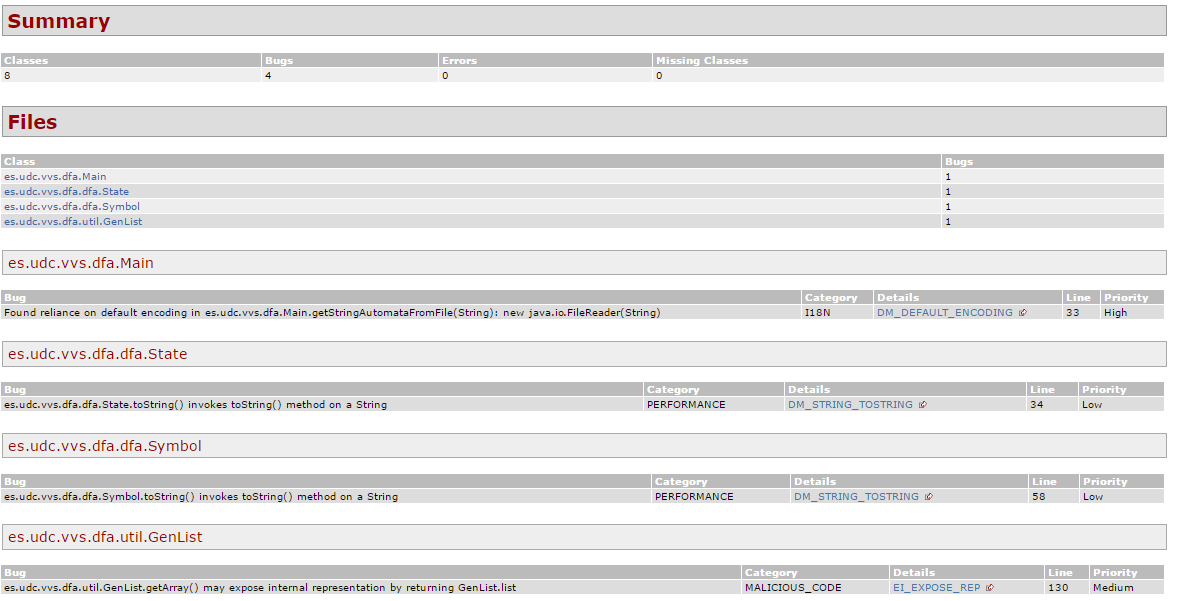
\includegraphics[width=15cm]{Imagenes/findBugs1.png} \\
	
	Después de identificar los errores, resolvemos los problemas mencionados y comprobamos el resultado:\\
	
	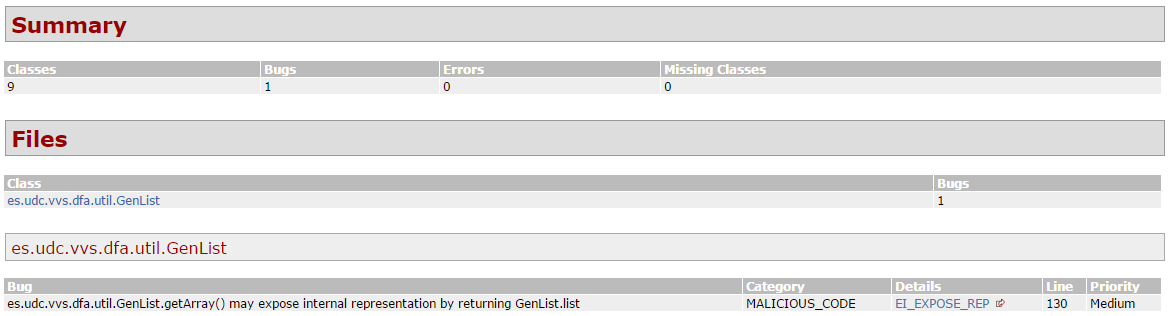
\includegraphics[width=15cm]{Imagenes/findBugs2.png} \\

	\textit{C:} El informe inicial de CppCheck tenía este aspecto: \\

	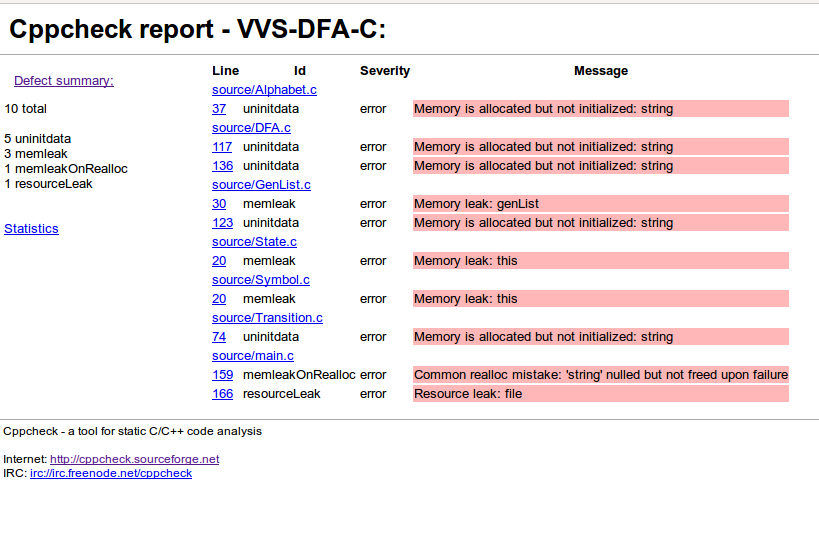
\includegraphics[width=15cm]{Imagenes/cppcheck.png}

	El informe actual se puede generar usando "make doc". Sólo queda el problema de \textit{resourceLeak}, el cual está referenciado en la issue 6 en el repositorio de GitHub. \\

\section{Estatísticas}

%\hint{Deben incluírse como mínimo:
  
  	\subsection{Número de errores encontrados diariamente y semanalmente.}
  	\textit{Java: }A partir de las pruebas de unidad con la herramienta junit, el mayor número de errores encontrados son después de realizar las pruebas de análisis de caja blanca (checkstyle y findbugs) y mutación de código (PITest). La tendencia después del punto álgido del 29/10/2016 (observar gráfica) a ir cerrando poco a poco las incidencias abiertas. 
  	
  	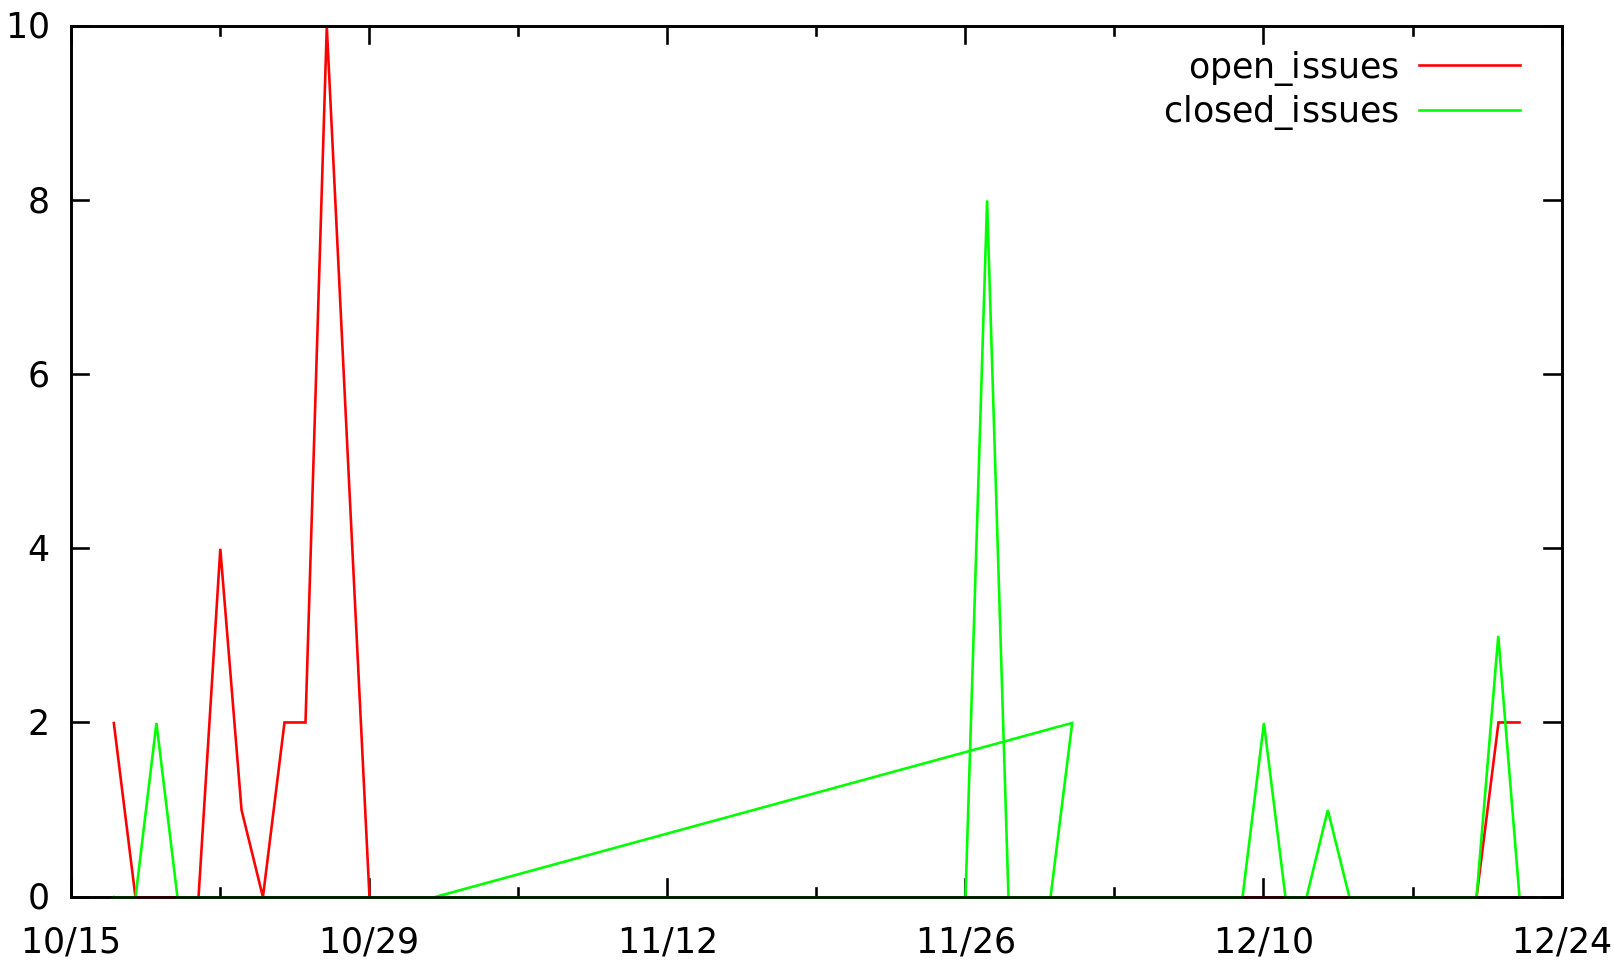
\includegraphics[width=15cm]{Imagenes/issues.png} \\
  	
  	Sin embargo, se puede observar que en las últimas semanas se volvieron a abrir issues debido a que se detectó que las pruebas realizadas no eran válidas según la cobertura. Por lo que se abren dos issues de herramientas y test pendientes de implementar para dar por completo por finalizado de testar la aplicación. \\
  	
  	\textit{C:} Por parte de este lenguaje, el ritmo de localización de pruebas empezó fuerte con la aplicación de las herramientas de CUnit, QuickCheck, y CppCheck, los cuales detectaron una cantidad sustancial de errores. Sin embargo, cometimos la equivocación de no empezar a cerrar issues hasta tener todos los tests implementados junto con las herramientas, lo cual considerando los problemas que hubo no fue la mejor de las ideas. Las issues se cerraron en Diciembre sin demasiadas complicaciones, el mes de distancia no es relevante con respecto a la dificultad de cerrarlas. \\ 
  	
  	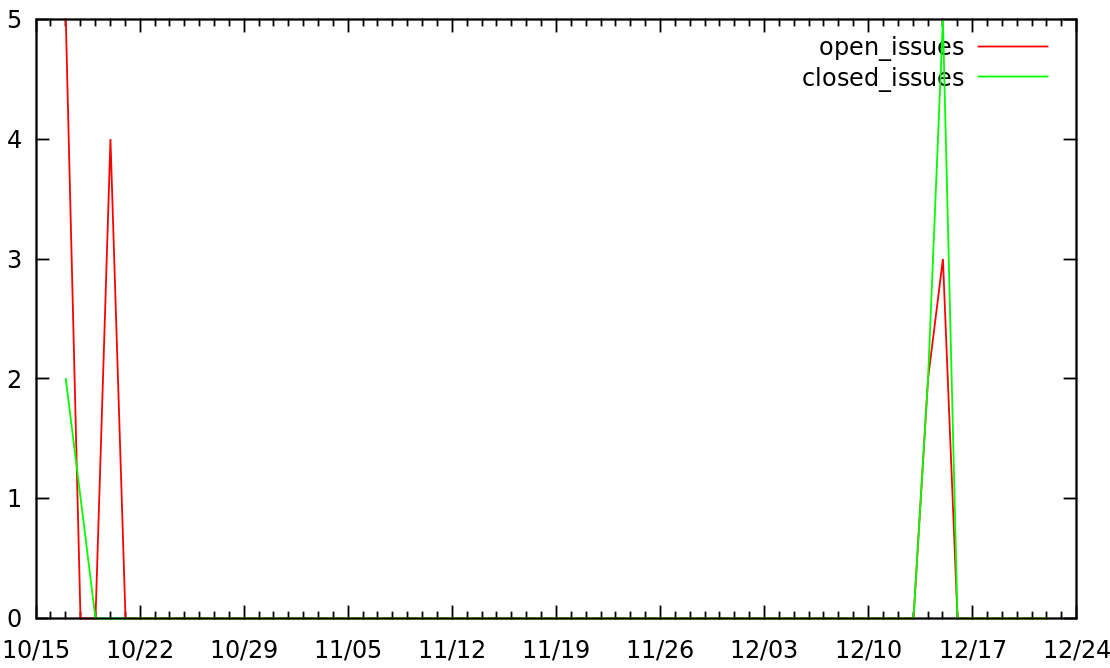
\includegraphics[width=15cm]{Imagenes/GraficoIssuesC.png} \\
  		
  	\subsection{Nivel de progreso de ejecución de las pruebas}
  	
  	\textit{Java: }Las pruebas diseñadas a priori fueron las pruebas iniciales de unidad, mockito y quickcheck.  	
  	A posteriori se fueron añadiendo las pruebas obtenidas de ejecutar las herramientas de análisis estático de caja blanca (CheckStyle), Herramienta de mutación de código (PITest).
  	
  	Podemos comprobar que con cobertura qué está al 68 por ciento y hemos diseñado pruebas para la clase DFA para mejorar la cobertura de nuestras pruebas. En una decisión inicial habíamos pensado en que estaban contenidas dentro de GenList pero por el resultado se comprueba qué es necesario realizar pruebas de las mismas. Faltarían por ejecutar. \\
  	
  	\textit{C:} Las pruebas diseñadas se pudieron implementar en su totalidad para los módulos que no necesitaron de un mock, siendo State, Symbol y GenList, los cuales tienen el 100\% de sus pruebas implementadas. El resto de módulos, sin embargo, no han implementado ninguna prueba debido a la imposibilidad de hacer funcionar los mocks en C. \\
  	
  	La cobertura fue satisfactoria para estos primeros módulos, alcanzando el 99.75\% del código cubierto. Se incluyeron pruebas para QuickCheck para comprobar que State y Symbol podían ser creados con cualquier cadena de caracteres sin problemas, se definieron funciones para liberación de memoria necesarios para poder hacer una cantidad significativa de tests repetidos con QuickCheck, y se incluyeron varias comprobaciones extra detectadas necesarias por las pruebas que diseñamos. 
  	
  	\subsection{Análisis del perfil de detección de errores}
  	%Análise do perfil de detección de erros. Trátase de que clasifiquedes as issues que tivestes no proxecto en función do compoñente ao que afectaron e o seu tipo (repasade a transparencia que explica ¿Qué es un bug? da primeira semana de clase deste bloque). O obxectivo é determinar se houbo partes do proxecto que concentraron máis problemas ca outras.
  	\textit{Java:} La mayoría de errores encontraros se encontraron sobre la clase GenList. Problemas con la lista de objetos y el buffer de objetos. \\
  	
  	\textit{C:} Los errores encontrados se concentraron principalmente en State y Symbol, dada la similitud de sus módulos y debido a su uso extensivo de cadenas de texto y reserva dinámica de memoria.
  	
	\subsection{Evaluación global del estado y calidad y estabilidad actual}
  	Actualmente se puede comprobar que el código es estable y las pruebas realizadas son correctas, sin embargo, eso no quiere decir de que no existan errores.
  	
  	\textit{Java:} En la definición de las pruebas decidimos no realizar pruebas sobre DFA porque considerábamos que estaban incluidas en GenList, sin embargo al validar con cobertura y con PIT(mutación testing) comprobamos que afecta negativamente a la validación de las pruebas. Se debería realizar más pruebas para una cobertura correcta del programa. Lo ideal sería obtener entre un 80 por ciento y 100 por cien de cobertura de las pruebas. 
  	
  	Decidimos no emplear las herramientas de GraphWalker, porque la ejecución de la aplicación es totalmente lineal y no nos generaría una máquina de estados útil para nuestras pruebas.
  	
  	Una cobertura del 68 por ciento no nos garantiza que existan bugs en el programa. Se podría considerar que consiguiendo realizar las pruebas de estrés y basadas en modelos y aumentando un poco la cobertura de las pruebas podríamos considerar que el programa está completamente validado y listo para utilizarse en algún entorno de producción. \\

	\textit{C:} Tuvimos problemas imprevistos con dos herramientas: Cmock y Milu. Al intentar utilizarlas, surgieron errores que no nos vimos capaces de solventar en tiempo, lo cual nos impidió su uso. Fue especialmente problemático lo de CMock, pues sin la posibilidad de hacer mocks nos quedó sin testear la mitad de los módulos. \\
	
	Por otro lado, las pruebas realizadas con el resto de herramientas dieron resultados satisfactorios, alcanzando el 99.75\% de cobertura en los módulos State y Symbol, y el 100\% con GenList, empleando de manera conjunta Unity y QuickCheck4c. \\
	
	Por parte de CppCheck, nos ayudó enormemente a localizar fugas de memoria por nuestro programa. Si bien en una ejecución normal no surgiría ningún problema, fue lo que nos permitió aumentar sustancialmente el número de pruebas a realizar con QuickCheck4c, pues no encontrábamos fallos de segmento debidos a la memoria huérfana que dejaban las pruebas.

\section{Otros aspectos de interés}

El equipo sufrió una baja (Javier López Moure) a mitad del proceso de pruebas, lo cual afectó a nuestra capacidad para realizar todas las pruebas sobre la aplicación. \\

\end{document}
